
\documentclass{article} % For LaTeX2e
\usepackage[final]{colm2026_conference}

\usepackage{microtype}
\usepackage{hyperref}
\usepackage{url}
\usepackage{booktabs}
\usepackage{graphicx}
\usepackage{amsmath,amsfonts,bm}
\usepackage{algorithm}
\usepackage{algorithmic}
\usepackage{subcaption}

\usepackage{lineno}

\definecolor{darkblue}{rgb}{0, 0, 0.5}
\hypersetup{colorlinks=true, citecolor=darkblue, linkcolor=darkblue, urlcolor=darkblue}


\title{Adjacent Latent Anchoring: Post-Hoc Representation Refinement\\for Masked Diffusion Language Models}

\author{
Ijin Yu \\
University of California, Berkeley \\
\texttt{ijinyu1113@berkeley.edu}
}

\newcommand{\fix}{\marginpar{FIX}}
\newcommand{\new}{\marginpar{NEW}}
\newcommand{\pmask}{p_{\text{mask}}}
\newcommand{\hmask}{\mathbf{h}_{\text{mask}}}
\newcommand{\hanchor}{\mathbf{h}_{\text{anchor}}}
\newcommand{\hblend}{\mathbf{h}_{\text{blend}}}
\newcommand{\deltaH}{\boldsymbol{\delta}}

\begin{document}

\ifcolmsubmission
\linenumbers
\fi

\maketitle

\begin{abstract}
Masked diffusion language models (MDMs) generate text by iteratively unmasking tokens, predicting each masked position using context gathered through the frozen model's transformer layers.
These layers perform general-purpose attention---handling long-range meaning, syntax, and world knowledge simultaneously---and we show empirically that their attention to local resolved tokens is severely diluted at high mask ratios (only 4\% of attention reaches nearby unmasked tokens when 95\% of positions are masked).
We introduce \textbf{Adjacent Latent Anchoring (ALA)}, a lightweight learned module that provides a dedicated pathway for local context extraction: for each masked position, ALA identifies nearby resolved tokens, computes corrections via a mixture-of-experts network, and aggregates them through learned attention---all without modifying the frozen base model or its decoding procedure.
Applied post-hoc to LLaDA-8B-Instruct, ALA improves GSM8K accuracy from 75\% to 81\% and MATH from 46\% to 50\%, while improving logical reasoning (4/4 vs.\ 3/4 baseline) and maintaining generation diversity.
A key finding is that per-step corrections compound across denoising: the optimal blending coefficient ($\alpha{=}0.05$) is $2\times$ lower than the training value, and corrected tokens become anchors for subsequent steps, creating an implicit dependency chain that amplifies small per-step improvements into large end-to-end gains.
ALA is orthogonal to sampling-level improvements such as ReMDM and PUNT, and can in principle be combined with them.
\end{abstract}


% ============================================================
\section{Introduction}
\label{sec:intro}
% ============================================================

Masked diffusion language models (MDMs) have emerged as a compelling alternative to autoregressive (AR) generation.
By framing text generation as iterative denoising of masked sequences, MDMs enable parallel token prediction, flexible generation order, and natural support for infilling tasks~\citep{austin2021structured, sahoo2024simple, nie2025llada}.
LLaDA~\citep{nie2025llada} scaled this paradigm to 8 billion parameters, matching LLaMA~3 8B on several benchmarks and demonstrating that MDMs can compete with AR models at scale.

At each denoising step, an MDM predicts every masked token using context gathered through its frozen transformer layers.
These layers perform general-purpose attention---handling long-range meaning, syntax, world knowledge, and local context all at once.
We analyze the base model's attention patterns and find that at high mask ratios---where MDMs spend most of their denoising trajectory---up to 89\% of attention weight at masked positions is absorbed by other \texttt{[MASK]} tokens, which all share identical embeddings and carry no useful information.
Only 4\% reaches nearby unmasked tokens (Section~\ref{sec:dilution}).
Moreover, masked positions that happen to allocate more attention to local unmasked tokens predict up to $8\times$ more accurately, demonstrating that the local signal exists but is underexploited.
This motivates a dedicated module for local context extraction.

Existing post-hoc methods for MDMs focus on either the \emph{decoding schedule}---which tokens to commit when---through remasking~\citep{shi2025remdm}, dependency testing~\citep{chen2025punt}, copula models~\citep{nisonoff2025copula}, energy-based correction~\citep{sun2025edlm}, and path planning~\citep{gat2025p2}; or on \emph{activation steering} using reference sequences~\citep{wang2026ilrr} or hand-designed intervention directions~\citep{turner2024steering, li2023iti}.
None provides a learned, general-purpose module for improving the per-step predictions themselves from the model's own hidden states.

We propose \textbf{Adjacent Latent Anchoring (ALA)}, a learned post-hoc module that provides a dedicated local context extraction pathway for masked positions.
For each masked position, ALA identifies nearby unmasked \emph{anchors}, computes pair-specific corrections via a mixture-of-experts (MoE) network, and aggregates them through learned attention---producing a position-specific hidden-state refinement that is added to the frozen base model's representations before the output projection.
ALA introduces no changes to the base model weights, training objective, or decoding algorithm.

A key property of ALA is that its corrections \emph{compound} across denoising steps.
At each step, corrected tokens are committed and become anchors for subsequent steps, creating an implicit dependency chain across the denoising trajectory.
This means even very small per-step corrections ($\alpha{=}0.05$) can cascade into substantial end-to-end improvements---while larger corrections ($\alpha{\geq}0.1$) destabilize generation as errors compound instead.

Our contributions are:
\begin{enumerate}
    \item \textbf{Architecture.} We introduce ALA, the first \emph{learned} post-hoc inference-time module for MDMs. Unlike sampling-level methods (ReMDM, PUNT) or methods requiring external AR models (Copula Diffusion, EDLM-AR), ALA learns to produce context-aware corrections from MDM hidden states alone.
    \item \textbf{Empirical gains.} Applied to LLaDA-8B-Instruct, ALA achieves +6\% on GSM8K (75\%$\to$81\%), +4\% on MATH (46\%$\to$50\%), and perfect logical reasoning (4/4 vs.\ 3/4), while improving generation diversity.
    \item \textbf{Correction compounding.} We show that the optimal inference-time $\alpha$ (0.05) is $2\times$ lower than the training $\alpha$ (0.1), and that performance degrades steeply at higher values. This reveals that per-step corrections compound across iterative denoising, analogous to learning rate sensitivity in gradient descent.
    \item \textbf{Attention dilution analysis.} We provide the first empirical characterization of attention dilution in MDMs: at high mask ratios, masked positions attend overwhelmingly to other \texttt{[MASK]} tokens. Positions with more local-unmasked attention predict $8\times$ more accurately, and ALA's corrections are net-positive across all attention regimes (5:1 correction-to-regression ratio), with the module extracting signal from local context that the diluted base attention underexploits.
\end{enumerate}


% ============================================================
\section{Background}
\label{sec:background}
% ============================================================

\subsection{Masked diffusion language models}

An MDM defines a forward (noising) process that progressively replaces tokens with \texttt{[MASK]}, and a reverse (denoising) process that recovers the original sequence.
Given a sequence $\mathbf{x} = (x_1, \ldots, x_L)$, the forward process at time $t$ produces $\mathbf{x}_t$ by independently replacing each token with \texttt{[MASK]} with probability $t$~\citep{austin2021structured, sahoo2024simple}.
A neural network $p_\theta(\mathbf{x}_0 \mid \mathbf{x}_t)$ is trained to predict the clean tokens from the noised sequence, factorized as:
\begin{equation}
    p_\theta(\mathbf{x}_0 \mid \mathbf{x}_t) = \prod_{i : x_{t,i} = \texttt{[MASK]}} p_\theta(x_{0,i} \mid \mathbf{x}_t)
    \label{eq:ci}
\end{equation}

This \textbf{conditional independence} factorization---each masked position predicted independently---is both the source of MDMs' parallelism and their primary limitation.
At generation time, a schedule determines how many tokens to unmask per step; at each step, the model predicts all masked positions, and the most confident predictions are committed~\citep{nie2025llada}.

\subsection{Why might general-purpose attention underexploit local context?}

In a transformer-based MDM, every \texttt{[MASK]} token enters the network with an identical embedding vector.
Through $L$ layers of self-attention, each masked position gathers context from both resolved and other masked positions, producing a final hidden state $\mathbf{h}_i^{(L)}$ that encodes its surrounding context.
This context propagation is powerful---it is the core mechanism by which MDMs make predictions---but it is also \emph{general-purpose}.
The same attention layers must simultaneously handle long-range semantic relationships, syntactic structure, world knowledge, and fine-grained local token dependencies.

We hypothesize three reasons why a small, dedicated module can improve on this general-purpose propagation:

\textbf{(1) Training objective.}
The model was trained with an independent per-position loss (Equation~\ref{eq:ci}): the gradient for position $i$ optimizes only ``predict token $i$ correctly,'' not ``extract maximally useful signal from position $i$'s nearest resolved neighbors.''
The attention patterns learned during training are good enough for each position's prediction, but not specifically tuned for local context extraction.

\textbf{(2) Attention dilution.}
Each attention head serves many functions across all positions and all mask ratios.
We verify this empirically in Section~\ref{sec:dilution}: at $\pmask{=}0.85$, masked positions allocate 79\% of attention to other \texttt{[MASK]} tokens, leaving only 8\% for local unmasked tokens within 10 positions.
A specialized module that attends \emph{only} to nearby resolved tokens, using a separate set of learned parameters, can focus its entire capacity on this one task.

\textbf{(3) Frozen output head.}
The output projection $W_{\text{out}}$ that maps hidden states to vocabulary logits is a fixed linear map.
A dedicated module can learn to produce perturbations specifically in directions that $W_{\text{out}}$ is sensitive to---shifting logits enough to change the argmax at critical positions, even when the perturbation is small in hidden-state space.

ALA intervenes after the base model computes $\mathbf{h}^{(L)}$ but before the output head projects to vocabulary logits.
By adding a small, position-specific correction derived from nearby resolved tokens, ALA can adjust predictions without modifying any base model parameters.


% ============================================================
\section{Method: Adjacent Latent Anchoring}
\label{sec:method}
% ============================================================

\subsection{Overview}

Given a partially-masked sequence at denoising step $t$, the frozen base model produces last-layer hidden states $\mathbf{H}^{(L)} \in \mathbb{R}^{L \times d}$.
For each masked position $i$, ALA:
\begin{enumerate}
    \item Identifies \textbf{anchor} positions: unmasked tokens within distance $r$ of position $i$.
    \item Computes a \textbf{pair-specific correction} $\deltaH_{ij}$ for each anchor $j$ via a mixture-of-experts network.
    \item \textbf{Aggregates} corrections across anchors using learned attention weights.
    \item \textbf{Blends} the aggregated correction into the hidden state: $\hblend_i = \mathbf{h}_i^{(L)} + \alpha \cdot \deltaH_i$.
\end{enumerate}
The blended hidden states are then projected to vocabulary logits through the frozen output head.
The entire process adds one forward pass through the lightweight ALA module per denoising step, with no changes to the decoding algorithm.

\subsection{Anchor identification}

For masked position $i$, we define its anchor set as:
\begin{equation}
    \mathcal{A}_i = \{j : x_{t,j} \neq \texttt{[MASK]},\ 0 < |i - j| \leq r\}
\end{equation}
where $r$ is the anchor range (we use $r{=}10$).
This local window captures the most relevant contextual tokens---those whose resolved values directly constrain what token should appear at position $i$.
As denoising progresses and more tokens are committed, the anchor set grows, providing increasingly rich local context.

\subsection{Mixture-of-experts correction}

For each (anchor, mask) pair $(j, i)$, we concatenate their hidden states and route through $K{=}8$ expert networks:
\begin{equation}
    \deltaH_{ij} = \sum_{k=1}^{K} w_k(\hmask_i) \cdot E_k([\hanchor_j;\, \hmask_i])
    \label{eq:moe}
\end{equation}
where $w_k(\hmask_i) = \text{softmax}(W_r \hmask_i)_k$ are soft routing weights computed from the mask token, $E_k$ is the $k$-th expert (a bottleneck MLP: $\mathbb{R}^{2d} \to \mathbb{R}^{d/2} \to \mathbb{R}^{d}$), and $[\cdot\,;\,\cdot]$ denotes concatenation.

The MoE design enables specialization: different experts can learn different types of corrections (e.g., syntactic agreement, numerical reasoning, entity tracking) while the router selects the appropriate mixture per token.
Expert output layers are zero-initialized so the module starts as identity (no correction).

\subsection{Learned attention aggregation}

When multiple anchors are available for a single masked position, we aggregate their corrections via learned attention:
\begin{equation}
    \deltaH_i = \sum_{j \in \mathcal{A}_i} \text{softmax}_j\!\left(\frac{\mathbf{q}_i^\top \mathbf{k}_j}{\sqrt{d_{\text{proj}}}}\right) \cdot \deltaH_{ij}
    \label{eq:attn}
\end{equation}
where $\mathbf{q}_i = W_q \hmask_i$ and $\mathbf{k}_j = W_k \hanchor_j$, with $d_{\text{proj}} = d/8 = 512$.
This mechanism allows the router to learn which anchors are most informative---nearby tokens carrying strong syntactic or semantic constraints receive higher weights than distant or less relevant ones.

\subsection{Residual blending}

The final correction is applied as a residual:
\begin{equation}
    \hblend_i = \mathbf{h}_i^{(L)} + \alpha \cdot \deltaH_i
    \label{eq:blend}
\end{equation}
where $\alpha$ is a scalar blending coefficient.
The blended hidden states are projected to logits via the frozen output head: $\text{logits}_i = W_{\text{out}} \hblend_i$.
Crucially, non-masked positions receive zero correction ($\deltaH_i = \mathbf{0}$ for $i \notin \text{masked}$), so ALA only modifies predictions at positions that need them.

\subsection{Training}

ALA is trained with a single-step masked prediction objective on the frozen base model's hidden states.

\paragraph{Data.}
We train on a mixture of Wikitext-103~\citep{merity2016wikitext}, GSM8K~\citep{cobbe2021gsm8k} (train split, 12$\times$ upsampled), and MATH~\citep{hendrycks2021math} (train split, 12$\times$ upsampled), yielding approximately 360K examples with ${\sim}50\%$ mathematical content.

\paragraph{Masking.}
For each training example, we sample $\pmask \sim \text{Uniform}(0.3, 1.0)$ and randomly mask that fraction of tokens.
Training across diverse mask ratios exposes the router to conditions analogous to different stages of iterative generation.

\paragraph{Pair construction.}
For each masked token, we identify all unmasked tokens within distance $r{=}10$.
Each (anchor, mask) pair is processed independently through the training router, which computes a correction $\deltaH$ and blends it: $\hblend = \hmask + \alpha \cdot \deltaH$.
The blended representation is projected through the frozen output head to produce logits.

\paragraph{Loss.}
Standard cross-entropy between predicted logits and ground-truth tokens at masked positions:
\begin{equation}
    \mathcal{L} = \mathbb{E}_{\pmask, \text{pairs}} \left[ -\log p(x_i^* \mid \hblend_i) \right]
\end{equation}

\paragraph{Optimization.}
AdamW~\citep{loshchilov2017adamw} with learning rate $5{\times}10^{-4}$, cosine annealing to $10^{-5}$, weight decay 0.01, gradient clipping at 1.0.
Training runs for 10K steps with effective batch size 32 (8 $\times$ 4 gradient accumulation) in bfloat16 mixed precision.
Training $\alpha$ is fixed at 0.1 (see Section~\ref{sec:alpha} for inference-time tuning).

\paragraph{Parameters.}
The ALA module adds approximately 206M trainable parameters (2.6\% of the 8B base model), comprising 8 expert MLPs (25M each), routing network, and Q/K projections.
The base model remains entirely frozen throughout training.


% ============================================================
\section{Experiments}
\label{sec:experiments}
% ============================================================

\subsection{Setup}

We evaluate ALA on LLaDA-8B-Instruct~\citep{nie2025llada} across eight evaluation dimensions.
Generation uses block-wise confidence-based unmasking with 256 steps, 256 generation tokens, and block length 32, following the LLaDA default configuration.
All generative evaluations use greedy decoding (temperature 0) unless otherwise noted.

\subsection{Main results}

\paragraph{Mathematical reasoning.}
Table~\ref{tab:main} shows end-to-end accuracy on GSM8K~\citep{cobbe2021gsm8k} (100 test samples) and MATH~\citep{hendrycks2021math} (50 test samples).
ALA improves GSM8K from 75\% to 81\% (+6 absolute) and MATH from 46\% to 50\% (+4 absolute).
These gains arise purely from better per-step predictions---the decoding algorithm is identical between baseline and router.

\begin{table}[t]
\begin{center}
\begin{tabular}{lcc}
\toprule
\textbf{Benchmark} & \textbf{Baseline} & \textbf{+ ALA} \\
\midrule
GSM8K (100) & 75.0\% & \textbf{81.0\%} \\
MATH (50) & 46.0\% & \textbf{50.0\%} \\
Logical Reasoning (4) & 3/4 & \textbf{4/4} \\
\bottomrule
\end{tabular}
\end{center}
\caption{End-to-end generation accuracy. ALA improves mathematical reasoning across benchmarks while recovering a logical reasoning failure (Triple Swap) that the baseline consistently gets wrong.}\label{tab:main}
\end{table}

\paragraph{Logical reasoning.}
We evaluate on four hand-crafted multi-step reasoning problems requiring state tracking (Triple Swap, Distractor, Relational, State Swap).
The baseline fails the Triple Swap problem (predicting ``cherry'' instead of ``banana'' after a sequence of swaps), while ALA correctly tracks the object transfers across all temperatures tested (0.0, 0.15, 0.3).
This demonstrates that ALA's corrections carry meaningful relational information.

\paragraph{Single-step mask prediction.}
On Wikitext-2 with $\pmask{=}0.15$, ALA improves prediction accuracy from 79.1\% to 81.9\% (+2.8 absolute), confirming that the router provides a genuine signal---not just noise that happens to help generation through stochastic effects.

\subsection{Mask prediction across ratios}

Table~\ref{tab:maskratio} shows accuracy and confidence improvements across mask ratios from 0.15 to 0.95.
ALA provides consistent gains at all ratios, with the largest accuracy improvement at $\pmask{=}0.85$ (+3.0\%) and monotonically increasing improvements from low to high masking.
This is expected: at high mask ratios (early denoising steps), there are fewer resolved tokens and more masked positions competing for context, so anchor-aware corrections are most valuable.

\begin{table}[t]
\begin{center}
\begin{tabular}{ccccc}
\toprule
$\pmask$ & Base Acc & Router Acc & $\Delta$Acc & $\Delta$Conf \\
\midrule
0.15 & 0.737 & 0.745 & +0.008 & +0.016 \\
0.30 & 0.663 & 0.679 & +0.015 & +0.018 \\
0.50 & 0.498 & 0.518 & +0.019 & +0.020 \\
0.70 & 0.303 & 0.326 & +0.023 & +0.019 \\
0.85 & 0.128 & 0.158 & +0.030 & +0.013 \\
0.95 & 0.040 & 0.058 & +0.018 & +0.005 \\
\bottomrule
\end{tabular}
\end{center}
\caption{Single-step mask prediction accuracy and confidence (probability of correct token) by mask ratio on Wikitext-2. ALA provides consistent improvements across all ratios, with the largest gains at high masking where anchor context is most scarce.}\label{tab:maskratio}
\end{table}

\subsection{Generation diversity}

We measure diversity across 5 samples per temperature on a creative writing prompt (Table~\ref{tab:diversity}).
At temperature 0, both models are deterministic.
At temperatures 0.15 and 0.3, ALA achieves \emph{lower} Jaccard similarity (more diverse outputs) than the baseline, indicating that the corrections do not collapse the output distribution but rather enable more varied, contextually appropriate completions.

\begin{table}[t]
\begin{center}
\begin{tabular}{ccccc}
\toprule
Temp & \multicolumn{2}{c}{Jaccard $\downarrow$} & \multicolumn{2}{c}{Unique Ratio $\uparrow$} \\
\cmidrule(lr){2-3} \cmidrule(lr){4-5}
 & Base & Router & Base & Router \\
\midrule
0.0  & 1.000 & 1.000 & 0.172 & 0.149 \\
0.15 & 0.612 & 0.540 & 0.275 & 0.276 \\
0.3  & 0.547 & 0.485 & 0.294 & 0.286 \\
\bottomrule
\end{tabular}
\end{center}
\caption{Generation diversity. Lower Jaccard = more diverse outputs. ALA maintains or improves diversity relative to the baseline at non-zero temperatures.}\label{tab:diversity}
\end{table}

\subsection{Entropy during denoising}

Figure~\ref{fig:entropy} shows the average entropy over masked positions at each denoising step.
ALA produces slightly lower entropy overall (mean 4.66 vs.\ 4.73 nats), indicating marginally more confident predictions.
The entropy curves closely track each other, confirming that ALA provides gentle corrections rather than aggressively reshaping the output distribution.

\begin{figure}[t]
\begin{center}

\includegraphics[width=\linewidth]{entropy_curve.png}
\end{center}
\caption{Per-step entropy during denoising. ALA (orange) produces marginally lower entropy than baseline (blue), with the difference most pronounced at block boundaries (steps 32, 64, 96) where new masked regions are exposed.}\label{fig:entropy}
\end{figure}


% ============================================================
\section{Analysis}
\label{sec:analysis}
% ============================================================

\subsection{Blending coefficient sensitivity}
\label{sec:alpha}

A critical finding is the sensitivity of generation quality to the blending coefficient $\alpha$.
We train with $\alpha{=}0.1$ but perform an inference-time sweep over $\alpha \in \{0.05, 0.10, 0.15, 0.20, 0.30, 0.50\}$ on 50 GSM8K samples (Figure~\ref{fig:alpha}).

\begin{figure}[t]
\begin{center}
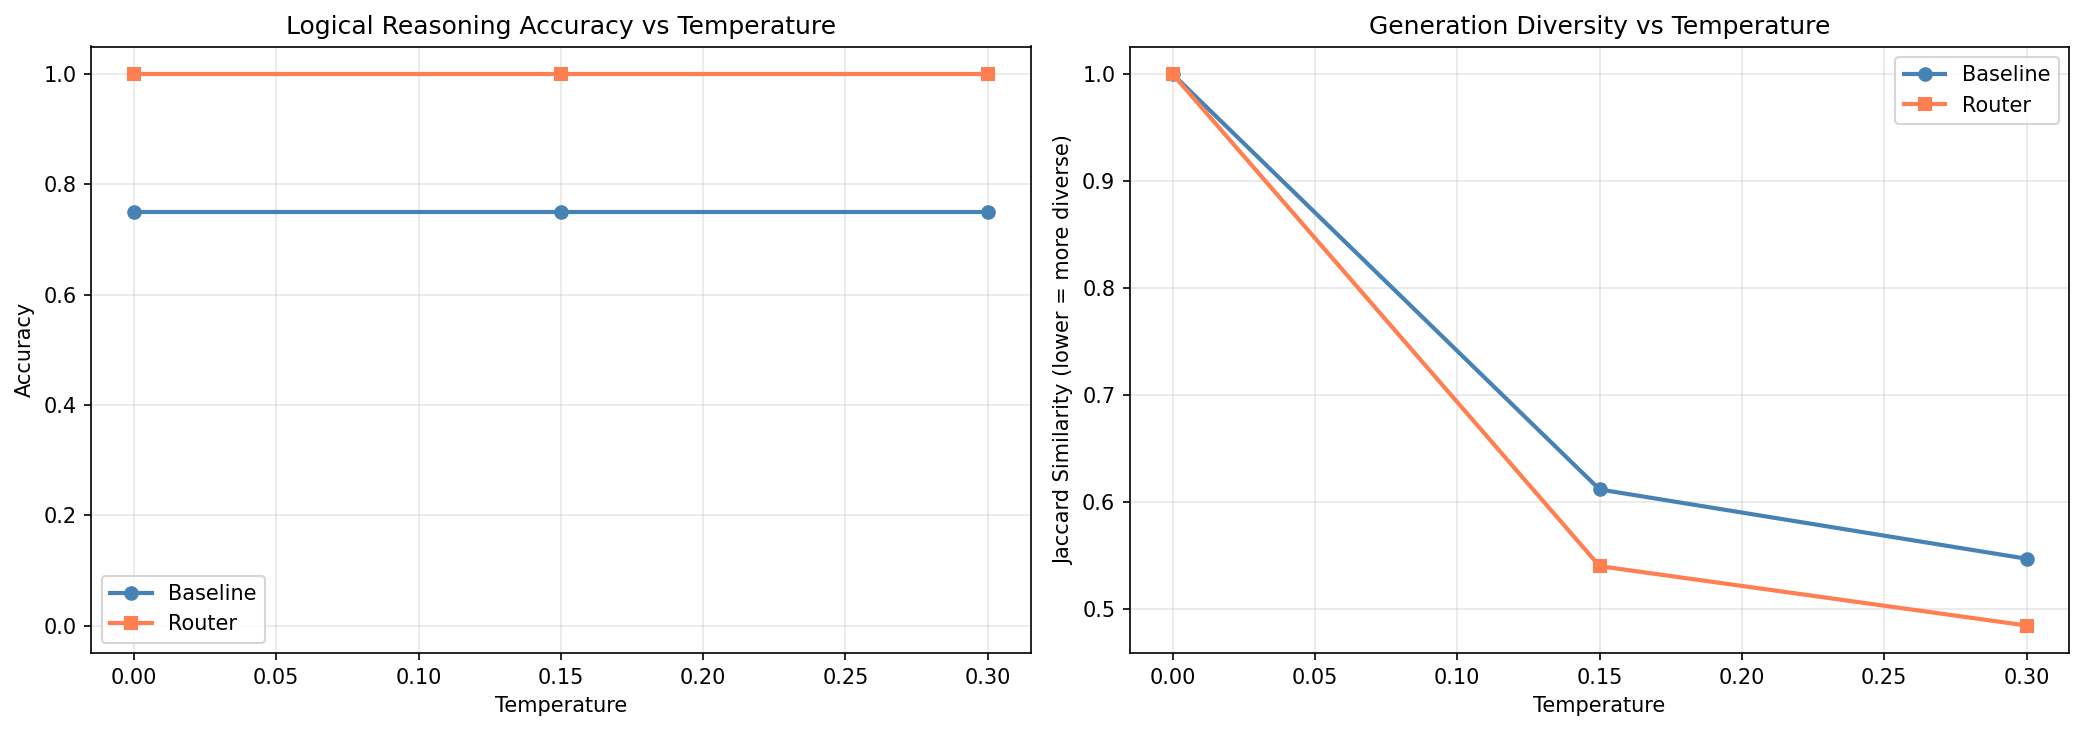
\includegraphics[width=0.85\linewidth]{sweep_summary.png}
\end{center}
\caption{\emph{Left:} Logical reasoning accuracy vs.\ temperature. ALA achieves 4/4 at all temperatures while baseline plateaus at 3/4. \emph{Right:} Generation diversity (Jaccard similarity) vs.\ temperature. ALA produces more diverse outputs at non-zero temperatures.}\label{fig:alpha}
\end{figure}

The results are striking: $\alpha{=}0.05$ achieves 80\% accuracy (vs.\ 70\% baseline), while $\alpha{=}0.10$ merely matches the baseline.
At $\alpha{\geq}0.15$, performance degrades rapidly, falling below the baseline by $\alpha{=}0.20$.

\paragraph{Why does optimal inference $\alpha$ differ from training $\alpha$?}
During training, $\alpha{=}0.1$ is applied to a \emph{single} correction step on clean context.
During generation, the same correction is applied at every one of 256 denoising steps, where each step operates on the model's \emph{own} (potentially erroneous) predictions.
Corrections compound: a slightly over-corrected token at step $t$ shifts the context for step $t{+}1$, which shifts $t{+}2$, and so on.
At $\alpha{=}0.05$, corrections are small enough to improve predictions without destabilizing this iterative process.
This is analogous to the learning rate in gradient descent: the optimal per-step learning rate decreases as the number of optimization steps increases.

\paragraph{Practical implication.}
The blending coefficient is a free parameter that can be tuned at inference time without retraining.
This decouples the router's learned \emph{correction direction} from its applied \emph{correction magnitude}.

\subsection{Attention dilution analysis}
\label{sec:dilution}

We extract attention weights from the base model's last 8 transformer layers by replacing the scaled dot-product attention with a manual computation that captures the weight matrix.
For each masked position, we measure the fraction of attention allocated to three categories: other \texttt{[MASK]} tokens, distant unmasked tokens, and local unmasked tokens (within distance $r{=}10$, matching ALA's anchor range).

\paragraph{Attention budget.}
Table~\ref{tab:attn_budget} shows the attention breakdown across mask ratios.
At $\pmask{=}0.15$, masked positions allocate 32\% of attention to local unmasked tokens---sufficient for effective prediction.
But at $\pmask{=}0.85$ (representative of early denoising), 79\% of attention goes to other \texttt{[MASK]} tokens and only 8.5\% reaches local unmasked tokens.
At $\pmask{=}0.95$, this drops to 4\%.
This dilution occurs because \texttt{[MASK]} tokens share identical input embeddings, producing similar Q/K projections that compete for attention mass via softmax normalization.

\begin{table}[t]
\begin{center}
\begin{tabular}{cccc}
\toprule
$\pmask$ & To \texttt{[MASK]} & To Local Unmask & To Distant Unmask \\
\midrule
0.15 & 0.143 & 0.321 & 0.536 \\
0.30 & 0.222 & 0.276 & 0.502 \\
0.50 & 0.312 & 0.229 & 0.460 \\
0.70 & 0.582 & 0.141 & 0.276 \\
0.85 & 0.789 & 0.085 & 0.127 \\
0.95 & 0.892 & 0.040 & 0.069 \\
\bottomrule
\end{tabular}
\end{center}
\caption{Attention budget at masked positions (averaged over last 8 layers, 20 Wikitext-2 samples). At high mask ratios, the vast majority of attention goes to uninformative \texttt{[MASK]} tokens.}\label{tab:attn_budget}
\end{table}

\paragraph{Local attention predicts accuracy.}
We pool masked positions across $\pmask \in \{0.50, 0.70, 0.85\}$ and bin them into quintiles by local-unmasked attention.
Positions in the lowest quintile (Q1, least local attention) achieve only 6.1\% prediction accuracy, while Q5 positions (most local attention) achieve 47.7\%---an $8\times$ gap.
This confirms that the local context signal \emph{exists} and is \emph{predictive}, but the base model's diluted attention does not consistently extract it.

\paragraph{ALA helps across all attention regimes.}
We additionally measure whether ALA flips predictions from wrong to right (corrections) or right to wrong (regressions) within each quintile (Table~\ref{tab:ala_correction}).
ALA achieves a 5:1 correction-to-regression ratio overall (185 corrections vs.\ 36 regressions across 6,035 positions).
The correction rate is highest at Q5 (5.0\%), where local unmasked tokens are available but the base model's general-purpose attention does not fully exploit them.
At Q1, ALA still provides net improvement (2.9\% corrections vs.\ 0.3\% regressions), though its impact is limited by the scarcity of local anchors---consistent with ALA's mechanism of extracting signal from nearby resolved tokens.

\begin{table}[t]
\begin{center}
\begin{tabular}{ccccc}
\toprule
Quintile & Base Acc & Router Acc & Corrections & Regressions \\
\midrule
Q1 (low attn) & 6.1\% & 8.6\% & 2.9\% & 0.3\% \\
Q2 & 18.2\% & 20.9\% & 3.0\% & 0.3\% \\
Q3 & 33.2\% & 34.7\% & 2.6\% & 1.1\% \\
Q4 & 46.8\% & 48.1\% & 1.9\% & 0.7\% \\
Q5 (high attn) & 48.8\% & 53.2\% & 5.0\% & 0.6\% \\
\bottomrule
\end{tabular}
\end{center}
\caption{ALA correction and regression rates by local-unmasked attention quintile. Positions are pooled across $\pmask \in \{0.50, 0.70, 0.85\}$, then binned by how much base-model attention each position allocates to nearby unmasked tokens. ALA is net-positive across all quintiles.}\label{tab:ala_correction}
\end{table}

\begin{figure}[t]
\begin{center}
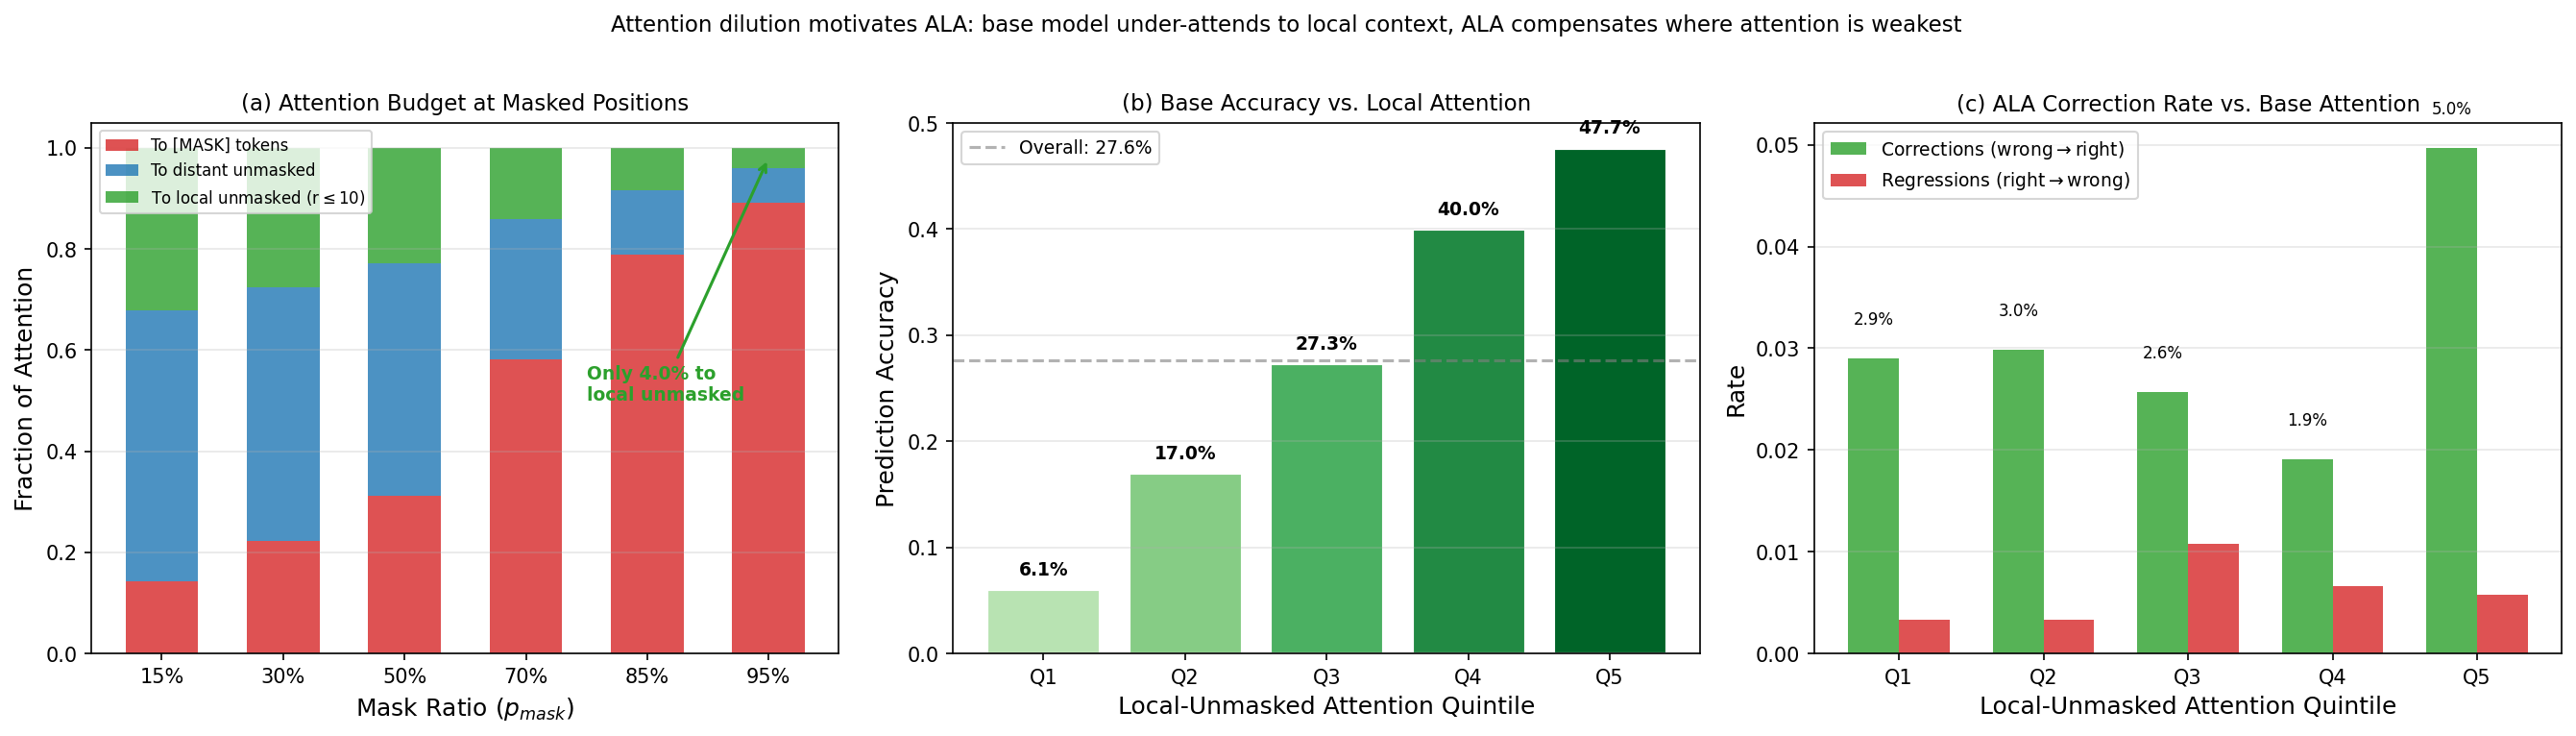
\includegraphics[width=\linewidth]{attention_dilution.png}
\end{center}
\caption{Attention dilution analysis. \textbf{(a)} At high mask ratios, masked positions attend overwhelmingly to other \texttt{[MASK]} tokens. \textbf{(b)} Positions with more local-unmasked attention predict more accurately. \textbf{(c)} ALA corrections (green) consistently outweigh regressions (red) across all attention quintiles.}\label{fig:attn_dilution}
\end{figure}

\subsection{Representation analysis}

Representation-level probing (Appendix~\ref{app:repr}) reveals that ALA consistently increases pairwise cosine similarity among masked positions ($+0.03$ on average) but does \emph{not} improve alignment with ground-truth hidden states.
The cohesion increase is expected---nearby masked positions share the same resolved anchors, so ALA pushes them in similar directions---while the lack of alignment improvement indicates that ALA operates through targeted \emph{logit-level} shifts rather than moving representations toward their ``correct'' values in hidden space.
Combined with the compounding mechanism (corrected tokens become anchors for subsequent steps), this explains why end-to-end gains (+6\% GSM8K) far exceed single-step accuracy improvements (+2--3\%).


% ============================================================
\section{Related work}
\label{sec:related}
% ============================================================

\paragraph{Masked diffusion language models.}
The foundation was laid by D3PM~\citep{austin2021structured} and generalized by MDLM~\citep{sahoo2024simple} and SEDD~\citep{lou2024discrete}.
LLaDA~\citep{nie2025llada} scaled to 8B parameters with competitive results.
Dream~\citep{dream2025} and Block Diffusion~\citep{arriola2025block} extended MDMs with knowledge transfer and hybrid architectures.
Recent RL-based post-training methods~\citep{ou2025d1} target MDM reasoning, but these modify the base model weights.
ALA is complementary: it operates on a frozen model at inference time.

\paragraph{Sampling-level improvements for MDMs.}
ReMDM~\citep{shi2025remdm} enables tokens to be re-masked and re-sampled via ancestral sampling.
Discrete Copula Diffusion~\citep{nisonoff2025copula} uses an external AR model to supplement dependency information.
PUNT~\citep{chen2025punt} uses conditional independence testing to identify conflicting tokens.
EDLM-AR~\citep{sun2025edlm} applies an AR energy function for correction.
Path planning~\citep{gat2025p2} optimizes token ordering.
These modify the \emph{decoding schedule}; ALA modifies the \emph{per-step predictions}---the two approaches are orthogonal.

\paragraph{Activation steering and representation engineering.}
ITI~\citep{li2023iti} shifts AR activations along truth-correlated directions.
ReFT/LoReFT~\citep{wu2024reft} learns task-specific representation interventions.
Activation addition~\citep{turner2024steering} steers behavior via mean-difference vectors.
ILRR~\citep{wang2026ilrr} steers MDM activations using reference sequences.
FK Steering~\citep{niehues2025fk} uses Feynman-Kac interacting particles for training-free guidance.
ALA differs from all of these in being \emph{learned from data} (vs.\ hand-designed or reference-dependent) and using a \emph{local anchor architecture} (vs.\ global steering directions).

\paragraph{Mixture of experts.}
The MoE paradigm~\citep{shazeer2017moe} enables parameter-efficient specialization.
ALA uses soft MoE routing where all experts process each input---a design choice that avoids the load-balancing issues of sparse routing while remaining computationally tractable due to the small number of experts ($K{=}8$) and the pair-level (not sequence-level) granularity of routing decisions.


% ============================================================
\section{Limitations and future work}
\label{sec:limitations}
% ============================================================

\textbf{Scale of evaluation.}
Our experiments use 100 GSM8K and 50 MATH samples rather than full test sets, and we evaluate on a single base model (LLaDA-8B-Instruct).
Scaling to full benchmarks and additional MDMs (Dream 7B, MDLM) would strengthen the claims.

\textbf{Sequential anchor processing.}
The inference router processes anchor-mask pairs with a loop over masked positions, which is slower than fully vectorized approaches.
Batched scatter/gather operations could substantially accelerate inference.

\textbf{Fixed anchor range.}
We use a fixed $r{=}10$ for all positions and denoising steps.
An adaptive range that expands as more tokens are resolved could capture longer-range dependencies.

\textbf{Combination with sampling methods.}
ALA is designed to be orthogonal to ReMDM, PUNT, and similar sampling-level methods.
Evaluating their combination is a natural next step---ALA improves per-step predictions while these methods improve the schedule of which predictions to commit.

\textbf{Mechanistic understanding.}
Our attention dilution analysis (Section~\ref{sec:dilution}) provides empirical motivation, and representation analysis shows ALA works through logit-level shifts rather than ground-truth alignment.
Deeper investigation---probing which expert specializations emerge, or analyzing which token categories benefit most from ALA---would further strengthen the theoretical grounding.


% ============================================================
\section{Conclusion}
\label{sec:conclusion}
% ============================================================

We introduced Adjacent Latent Anchoring (ALA), a learned post-hoc module that provides a dedicated local context extraction pathway for masked diffusion language models.
We show that the general-purpose attention in frozen MDMs suffers from severe attention dilution at high mask ratios---up to 89\% of attention is absorbed by uninformative \texttt{[MASK]} tokens---and that a small specialized module (2.6\% of base model parameters) can compensate by providing a dedicated local context pathway, producing meaningful end-to-end gains (+6\% GSM8K, +4\% MATH) without modifying the base model or decoding procedure.
A key finding is that per-step corrections compound across iterative denoising, making the blending coefficient critical: the optimal value ($\alpha{=}0.05$) is $2\times$ lower than the training setting, with performance degrading rapidly at higher values.
Attention analysis reveals that masked positions allocate the vast majority of attention to uninformative \texttt{[MASK]} tokens at high mask ratios, empirically grounding ALA's motivation, while the mechanism operates through logit-level adjustments amplified by iterative denoising.
As the first learned inference-time module for MDMs, ALA opens a design axis orthogonal to existing sampling-level improvements and can in principle be composed with them.

% ============================================================

\section*{Reproducibility statement}

All experiments use publicly available models (LLaDA-8B-Instruct) and datasets (GSM8K, MATH, Wikitext).
The ALA module architecture, training procedure, and hyperparameters are fully specified in Section~\ref{sec:method}.
Code will be released upon publication.


\bibliography{colm2026_conference}
\bibliographystyle{colm2026_conference}

\appendix

\section{Architecture details}
\label{app:arch}

Table~\ref{tab:arch} provides the complete architectural specification.

\begin{table}[h]
\begin{center}
\begin{tabular}{ll}
\toprule
\textbf{Component} & \textbf{Specification} \\
\midrule
Base model & LLaDA-8B-Instruct (frozen) \\
Hidden dimension $d$ & 4096 \\
Number of experts $K$ & 8 \\
Expert bottleneck & $2d \to d/2 \to d$ (GELU) \\
Expert init & Zero-init output layer \\
Routing & Softmax over $W_r \hmask_i \in \mathbb{R}^K$ \\
Q/K projection dim & $d/8 = 512$ \\
Anchor range $r$ & 10 \\
Blending $\alpha$ (train) & 0.1 \\
Blending $\alpha$ (inference) & 0.05 \\
Total ALA parameters & 206M (2.6\% of base) \\
\midrule
\textbf{Training} & \\
\midrule
Optimizer & AdamW (lr=$5{\times}10^{-4}$, wd=0.01) \\
Schedule & Cosine annealing to $10^{-5}$ \\
Steps & 10,000 \\
Effective batch size & 32 (8 $\times$ 4 accum) \\
Mask ratio & $\pmask \sim U(0.3, 1.0)$ \\
Max pairs/batch & 2048 (subsampled) \\
Precision & bfloat16 \\
Data & Wiki-103 + GSM8K$\times$12 + MATH$\times$12 \\
\bottomrule
\end{tabular}
\end{center}
\caption{Complete ALA architecture and training specification.}\label{tab:arch}
\end{table}

\section{Representation analysis}
\label{app:repr}

Table~\ref{tab:mechinterp} shows the full breakdown of ALA's effect on hidden-state geometry across mask ratios.
Figure~\ref{fig:cossim} shows the pairwise cosine similarity analysis, and Figure~\ref{fig:twopanel} provides the joint view of pairwise similarity and ground-truth alignment.

\begin{table}[h]
\begin{center}
\begin{tabular}{ccc}
\toprule
$\pmask$ & $\Delta$ Pairwise & $\Delta$ Alignment \\
\midrule
0.15 & +0.030 & $-$0.002 \\
0.30 & +0.032 & $-$0.002 \\
0.50 & +0.036 & $-$0.001 \\
0.70 & +0.036 & $-$0.001 \\
0.85 & +0.028 & +0.001 \\
0.95 & +0.007 & +0.001 \\
\bottomrule
\end{tabular}
\end{center}
\caption{Representation analysis. ALA consistently increases pairwise hidden-state similarity (``cohesion'') but does not measurably improve alignment with ground-truth representations.}\label{tab:mechinterp}
\end{table}

\begin{figure}[h]
\begin{center}

\includegraphics[width=0.85\linewidth]{cosine_sim_by_mask_ratio.png}
\end{center}
\caption{Pairwise cosine similarity of masked-position hidden states by mask ratio. ALA (orange) consistently produces more similar representations than the baseline (blue).}\label{fig:cossim}
\end{figure}

\begin{figure}[h]
\begin{center}
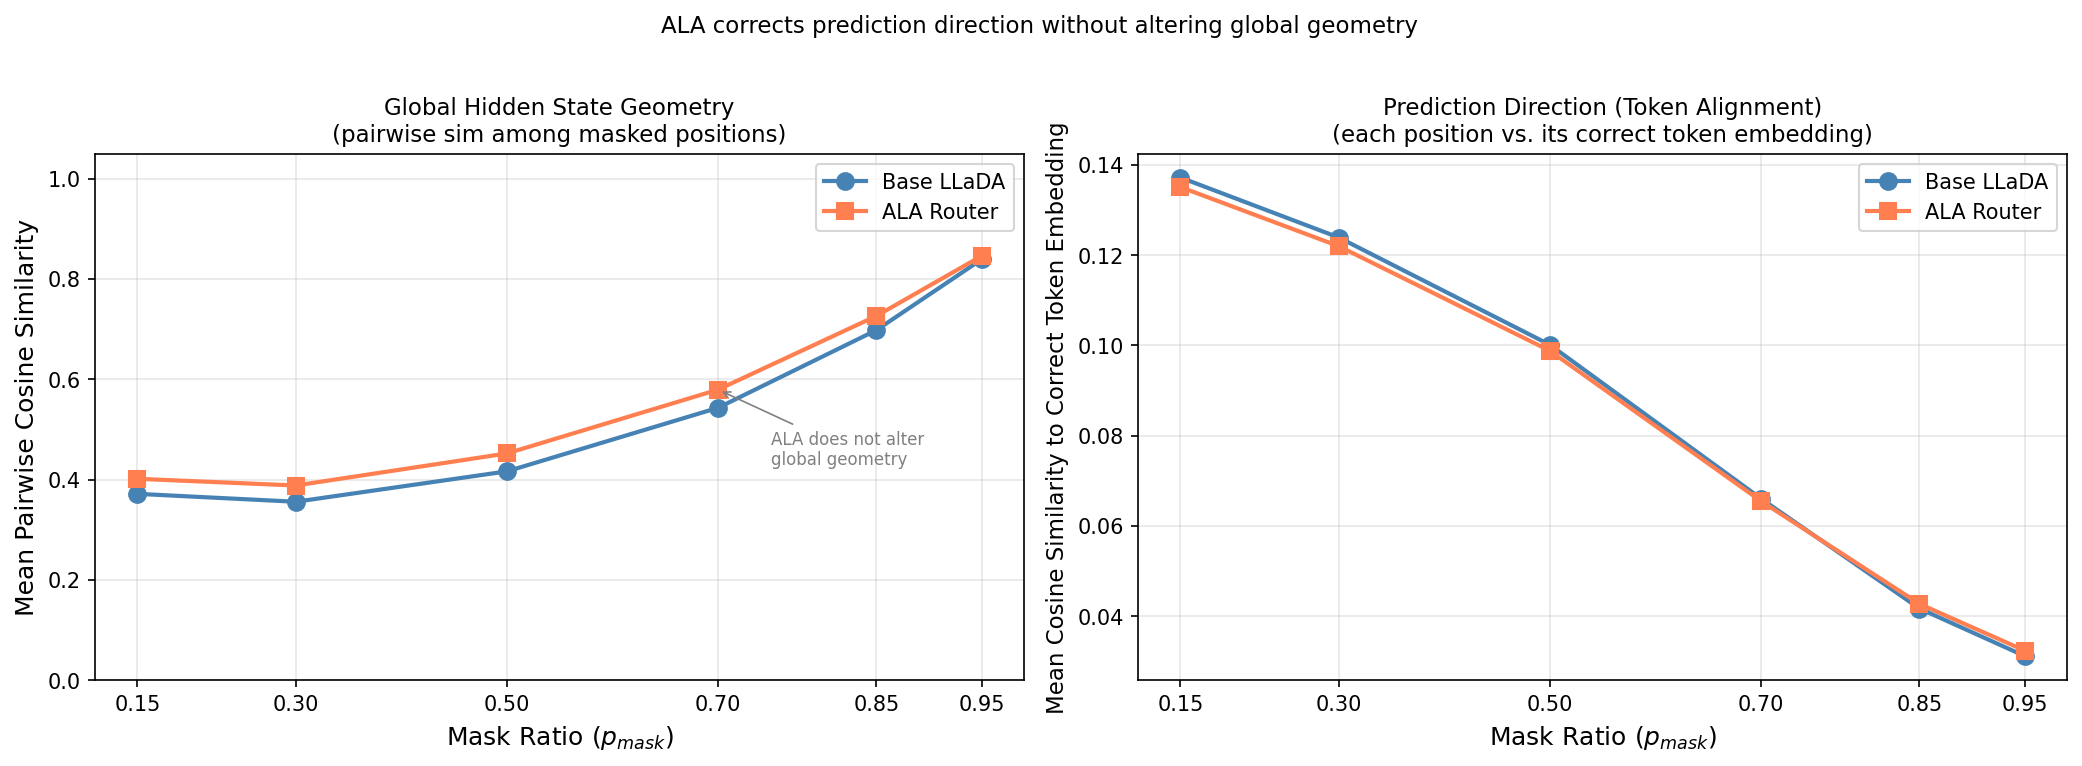
\includegraphics[width=0.85\linewidth]{two_panel_symmetry_vs_alignment.png}
\end{center}
\caption{\emph{Left:} Pairwise cosine similarity increase from ALA. \emph{Right:} Ground-truth alignment change from ALA. The router increases cohesion but does not improve alignment.}\label{fig:twopanel}
\end{figure}


\section{Alpha sweep details}
\label{app:alpha}

Full alpha sweep results on 50 GSM8K samples:

\begin{table}[h]
\begin{center}
\begin{tabular}{cc}
\toprule
$\alpha$ & GSM8K Accuracy \\
\midrule
0.00 (baseline) & 70\% \\
0.05 & \textbf{80\%} \\
0.10 & 70\% \\
0.15 & 56\% \\
0.20 & 42\% \\
0.30 & 26\% \\
0.50 & 14\% \\
\bottomrule
\end{tabular}
\end{center}
\caption{Alpha sweep on 50 GSM8K samples. Performance peaks at $\alpha{=}0.05$ and degrades steeply for higher values, demonstrating the compounding effect of corrections across 256 denoising steps.}\label{tab:alpha}
\end{table}


\section{Logical reasoning test cases}
\label{app:logic}

The four reasoning prompts used in evaluation:

\begin{enumerate}
    \item \textbf{Triple Swap.} ``Alice has an apple, Bob has a banana, and Charlie has a cherry. Alice swaps with Bob. Then Bob swaps with Charlie. Now, Alice has the \underline{\hspace{1cm}}'' (Expected: banana)
    \item \textbf{Distractor.} ``A gold coin is in the red box. A silver coin is in the blue bag. I replace the gold coin with a copper coin. The red box now has the \underline{\hspace{1cm}}'' (Expected: copper)
    \item \textbf{Relational.} ``The mountain is taller than the hill. The building is shorter than the hill. The shortest object is the \underline{\hspace{1cm}}'' (Expected: building)
    \item \textbf{State Swap.} ``I have a box and a bag. The ball is in the box. The key is in the bag. I swap them. The bag now has the \underline{\hspace{1cm}}'' (Expected: ball)
\end{enumerate}

The baseline consistently fails Triple Swap (predicting ``cherry'' instead of ``banana''), suggesting difficulty tracking state through multiple operations.
ALA correctly resolves all four at temperatures 0.0, 0.15, and 0.3.

\end{document}
